\begin{center}
    \vspace{2cm} 
    {\Huge \bfseries Maio} \\ 
    \vspace{1cm} 
\end{center}

\subsection*{Introdução}
Realizamos um circuito real simples que responde à aproximação de um objeto por meio do sensor ultrassônico, alternando as cores dos LEDs conforme o estado do programa, tocando melodia com buzzer passivo e girando o micro servo para simular o alimento sendo despejado.

Para o próximo mês, focaremos em estudar os componentes necessários para construção do Alimentador e como será implementado de fato, saindo da fase de testes e organizando melhor o trabalho.
\subsection*{Programa}
Utilizamos a extensão PlatformIO para o VS Code para criar e gerenciar o projeto. Ela oferece suporte a diversos \textit{frameworks} (no caso, o Arduino), além de possibilitar organização modular, depuração de código, compilação e injeção do programa na memória do microcontrolador.

Dessa forma, aprendemos sobre o \href{https://www.youtube.com/watch?v=B_Ysdv1xRbA&t=8s}{PWM}, uma forma de simular saída analógica, para gerar efeito de pulsação nos LEDs. Também, estudamos o funcionamento do sensor, do servo e do buzzer e como utilizar as bibliotecas nativas para escrever o algoritmo e montar o circuito.
\bigbreak

Main: 
\begin{itemize}
    \item Fase setup (roda apenas na inicialização do programa):
    ocorre a definição de cada pino do Arduino utilizado (\textbf{INPUT} ou \textbf{OUTPUT}) e o acoplamento do servo; a comunicação serial é inicializada, permitindo transferência de dados entre o programa e o computador; checa e alerta se há objeto próximo, exigindo a retirada.
    \item Fase loop:
    pulsa os LEDs na cor azul, realiza repetidamente a leitura do sensor e gera saída de texto informativo no monitor serial, checando se há objeto próximo para a ativação do sistema (mudança de brilho dos LEDs, melodia do \textit{buzzer} e rotação do servo).
\end{itemize}

\newpage
\lstinputlisting[title={main.cpp}]{./codes/main.cpp}
\bigbreak

O projeto completo pode ser visto no repositório do Github: \href{https://github.com/Ashylll/ieee-alimentador.git}{ieee-alimentador}

\newpage
\subsection*{Circuito}
O Arduino Uno, conectado ao computador por um cabo USB A/B, é utilizado como fonte de alimentação para o Micro Servo Motor SG90 e o sensor ultrassônico HC-SR04. O brilho dos LEDs, a frequência do \textit{buzzer}, o acionamento do pino \textit{Trig} (gatilho) do sensor e a ativação do motor ocorrem conforme a lógica do programa, o qual envia sinais \textbf{HIGH} (5V) ou \textbf{LOW} (0V) aos pinos de \textbf{OUTPUT}. O único sinal de \textbf{INPUT} recebido é do pino \textit{Echo} do sensor. Por fim, cada LED se conecta em série com um resistor de 330$\Omega$ e todos os componentes estão ligados ao pino GND (terra) do Arduino, fechando devidamente o circuito. Nota-se que os LEDs devem ser ligados a pinos PWM da placa (sinalizados por $\sim$) e que a biblioteca Servo desabilita essa função nos pinos $\sim$9 e $\sim$10.
\vspace{1.4cm}
\begin{figure}[h]
        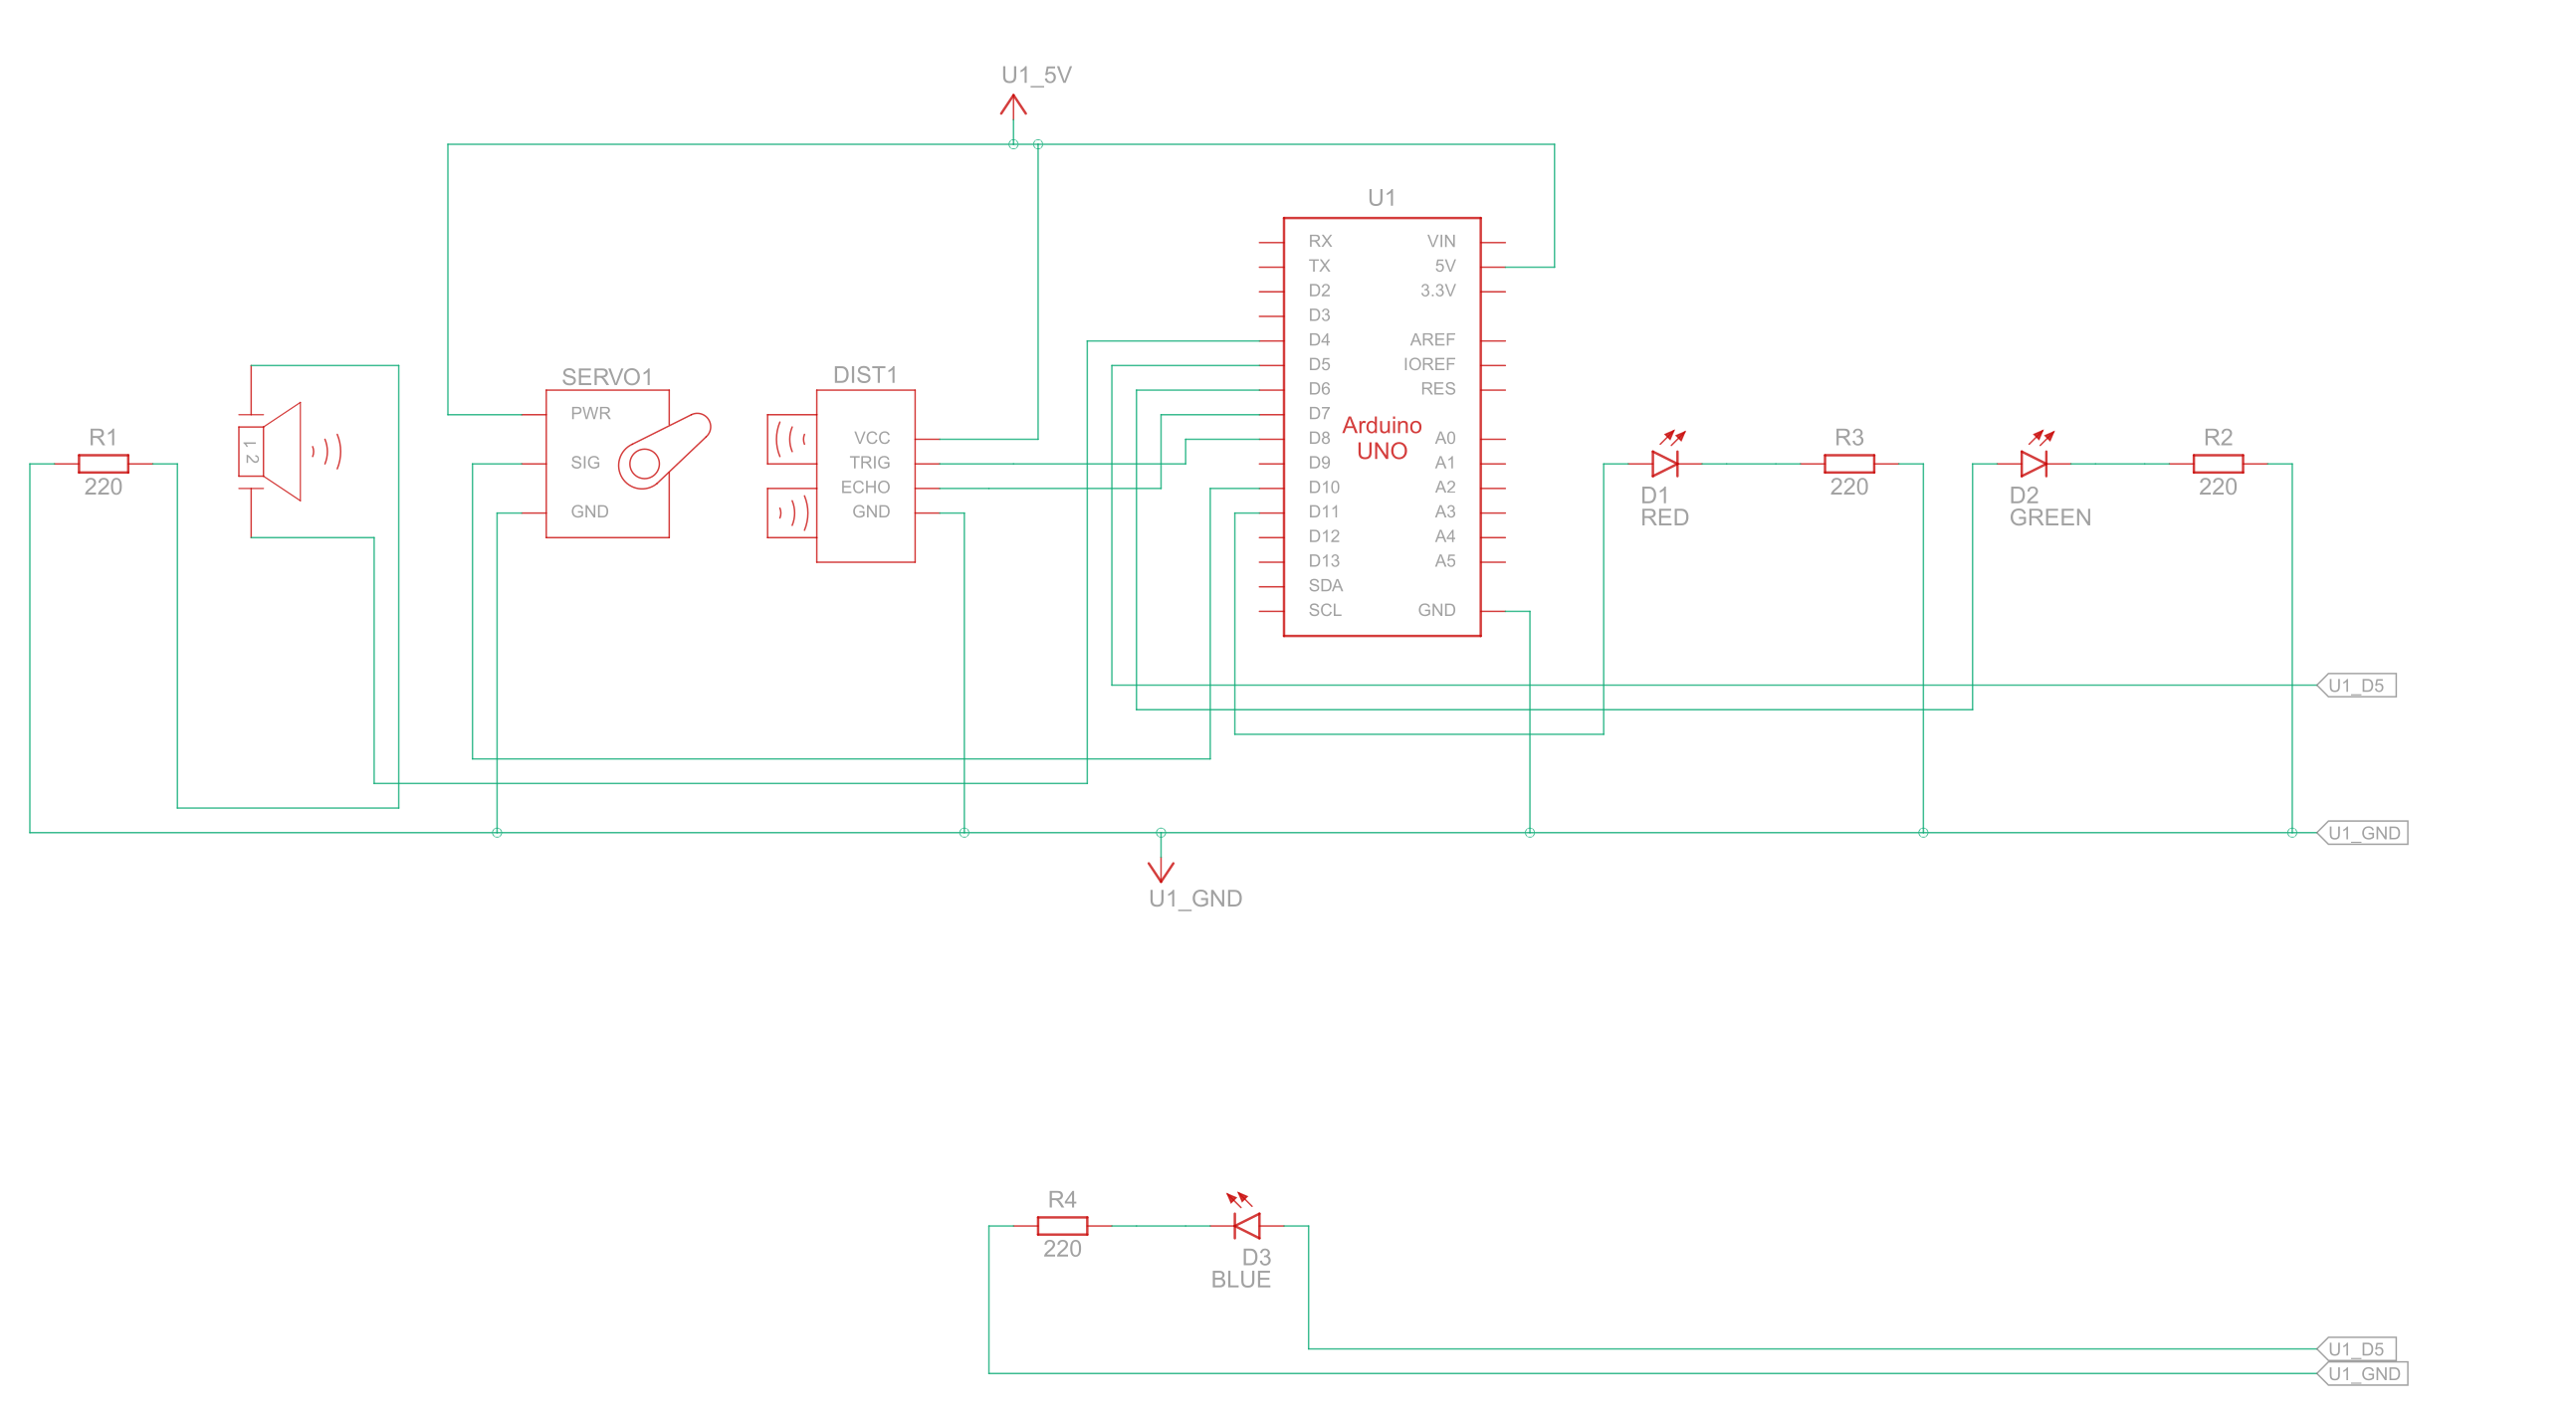
\includegraphics[width=\textwidth]{./figs/esquema.png}
        \caption* {Visão esquemática do circuito}
\end{figure}
\bigbreak
Obs.: utilizamos LEDs vermelho, verde e azul para simular o LED RGB.

\begin{figure}[htbp]
        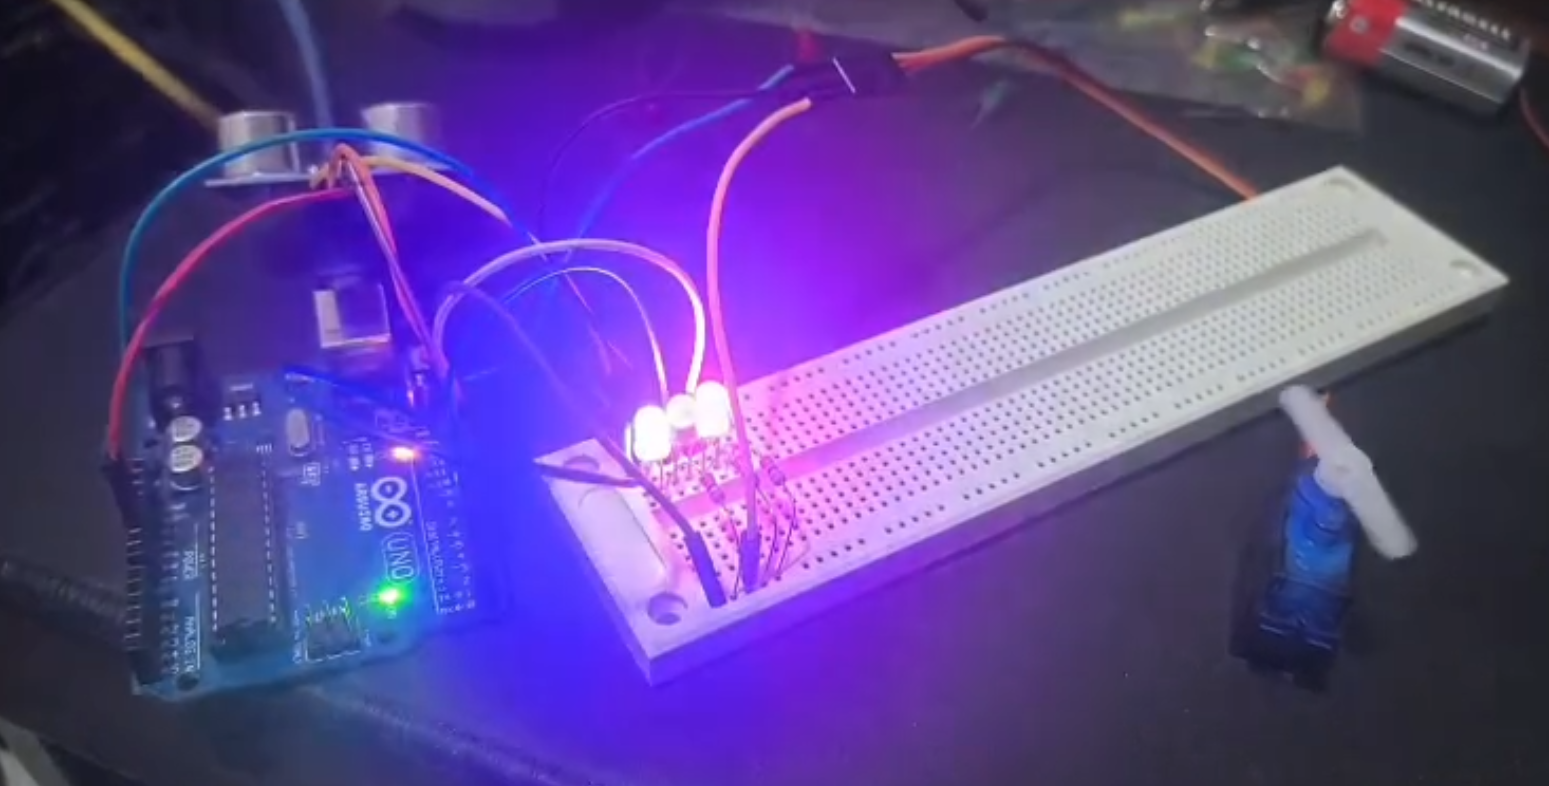
\includegraphics[width=\textwidth]{./figs/prototipo-foto.png}
        \caption* {Foto: servo voltando à posição de repouso quando o programa muda de estado (roxo $=$ comendo)}
\end{figure}

\newpage
\subsection*{Estudo e planejamento}
Este protótipo serviu apenas como base para aprender e praticar a lógica da programação e a montagem do circuito voltados ao Arduino. Agora, pretendemos expandir e esquematizar o Alimentador para termos um planejamento sólido sobre o caminhar do projeto e o resultado final.\\

Referências de estudo para a continuação do trabalho:
\renewcommand{\labelitemi}{$\cdot$}
\begin{itemize}
    \item \href{https://www.youtube.com/watch?v=fHzWA9GLAkc}{Parafuso de Arquimedes}
    \item \href{https://www.youtube.com/watch?v=o4i_vMHziBw}{Motor de passo}
    \item \href{https://www.micro-tess.com/wheatstone-bridge/}{Ponte de Wheatstone}
    \item \href{https://docs.soldered.com/hx711/overview/}{Módulo amplificador}
    \item \href{https://www.youtube.com/watch?v=dNiVZBTvwxs}{Células de carga} 
\end{itemize}